\documentclass[GBK,winfonts,a4paper,10pt]{ctexart}
\usepackage{fancyhdr}
\usepackage{indentfirst}
\usepackage{graphics}
\usepackage{enumerate}
\usepackage{framed}
\usepackage{amsmath}
\usepackage{graphicx}
\usepackage{setspace}
\usepackage{hyperref}
\usepackage{mdwlist}
\usepackage{algorithm}
\usepackage{algorithmic}
\usepackage{listings}
\usepackage{xcolor}
\lstset{numbers=left, numberstyle=\small, keywordstyle=\color{blue!70}, commentstyle=\color{red!50!green!50!blue!50}, frame=shadowbox, rulesepcolor=\color{red!20!green!20!blue!20},escapeinside=``, xleftmargin=2em,xrightmargin=2em, aboveskip=1em}
\usepackage{geometry}

\newcommand{\tabincell}[2]{\begin{tabular}{@{}#1@{}}#2\end{tabular}}%
       
\lstdefinestyle{customc}{
  belowcaptionskip=1\baselineskip,
  breaklines=true,
  frame=single,
  xleftmargin=\parindent,
  language=C,
  showstringspaces=false,
  basicstyle=\fontsize{8pt}{8pt}\ttfamily,
  keywordstyle=\bfseries\color{green!40!black},
  commentstyle=\itshape\color{purple!40!black},
  identifierstyle=\color{blue},
  stringstyle=\color{orange},
  tabsize=4,
  numbers=none,
}

\lstset{escapechar=@,style=customc}

\pagestyle{fancy}
\hypersetup{pdfborder=0 0 0}

\usepackage{clrscode}

\usepackage{latexsym}

\begin{document}

\rhead{}
\lhead{}
\cfoot{\thepage}
\renewcommand{\footrulewidth}{0.4pt}
%\renewcommand{\thesection}{}
\renewcommand{\algorithmicrequire}{\textbf{Input:}}
\renewcommand{\algorithmicensure}{\textbf{Output:}}
\setlength{\tabcolsep}{2pt}

\setlength{\parindent}{2em}

\thispagestyle{fancy}



\title{Operating System MIT 6.828 JOS Lab2 Report}
\author{Computer Science \\ ChenHao(1100012776) }
\date{\today}
\maketitle

\thispagestyle{fancy}

\tableofcontents

\newpage

\begin{section}{Part 1: Physical Page Management}

\begin{subsection}{Exercise 1}
\par
这个Lab意在让我们填充代码使得JOS能够正确使用新的的页寻址,由于具体寻址是由硬件实现的,对于内核的开发者需要做的只是做好内存的页的管理以及填写好初始Page Directory以及Page Table的值,之后将cr3指向我们新构建的表头,这样就可以使用新的页寻址了。
\par
需要注意的是在这段代码开始前我们就已经开始使用了页寻址了,因此代码不可避免地需要进行虚拟地址的转化,因此在代码中要保持清醒的头脑什么时候需要使用物理地址什么时候需要使用虚拟地址。
\begin{subsubsection}{boot\_alloc()}
\par 
直接ROUNDUP分配即可,注意要时刻保持nextfree对齐PGSIZE。
\par
end是什么?end是linker在链接的时候确定,其指向kernel的bss段的末尾。即kernel所使用的下一个空间的地址。end是指向虚拟地址的指针。
\begin{lstlisting}[language=C]
static void *
boot_alloc(uint32_t n)
{
	static char *nextfree;	// virtual address of next byte of free memory
	char *result;
	
	if (!nextfree) {
		extern char end[];
		nextfree = ROUNDUP((char *) end, PGSIZE);
	}
	
    result = nextfree;
    nextfree = ROUNDUP(nextfree + n, PGSIZE);

	return result;
}
\end{lstlisting}
\end{subsubsection}

从inc\textbackslash memlayout.h中可以知道JOS使用struct PageInfo 以及 page\_free\_list 来管理每个page,对于管理pages实际是一个链表,每个page保存其被引用的次数(pp\_ref)以及在链表中下一个free\_page的地址(pp\_link,仅当当前页为free\_page才有效),page\_free\_list指向空页链表的头部。

\begin{subsubsection}{mem\_init() (only up to call to check\_page\_free\_list(1))}
\par
需要建npages个PageInfo来管理pages.
\begin{lstlisting}[language=C]
pages = (struct PageInfo *) boot_alloc(npages * sizeof(struct PageInfo));
\end{lstlisting}

\end{subsubsection}

\begin{subsubsection}{page\_init()}
\par
page\_init为初始化整个内存空间,并建立空闲页的链表数据结构。PageInfo为页管理的数据结构。
\par
需要知道哪些位置的物理内存是不能被使用的,注释中提到了第0页和IO hole([IOPHYSMEM, EXTPHYSMEM))是不能用来分配的,而对于[EXTPHYSMEM, ...)需要确定哪些是不可以使用的。EXTPHYSMEM恰好就是1MB的位置,从Lab1中我们已经知道Kernel的代码和数据和栈都存放在了进接着1MB的位置,而extern char end[]恰好是kernel存放的最后的地址(这里是虚拟地址,实际的物理地址为end - KERNBASE)。而由mem\_init()中可以知道,初始分配了两页的空间给Initial Page Directory和PageInfo,这都是存放在紧接着char* end的连续的页中。因此第0页,以及IOPHYSMEM到char* end之后的已经使用的页均是不可分配的页,其余均是可行的。这里有个小的技巧,boot\_alloc(0)返回下一个未使用的内存的虚拟地址,因此可以直接计算得到不可分配页的最后的页编号。
\begin{lstlisting}[language=C]
void
page_init(void)
{
    page_free_list = NULL;
    size_t i;
	size_t nf_lb = IOPHYSMEM / PGSIZE;
    size_t nf_ub = PADDR(boot_alloc(0)) / PGSIZE;
    for (i = 0; i < npages; i++) {
        if (i != 0 && (i < nf_lb || i >= nf_ub)) {
		    pages[i].pp_ref = 0;
            pages[i].pp_link = page_free_list;
		    page_free_list = &pages[i];
        } else {
            pages[i].pp_ref = 1;
            pages[i].pp_link = NULL;
        }
	}
}
\end{lstlisting}
\end{subsubsection}

\par
page\_alloc和page\_free都只需要进行指针操作,调整page\_free\_list和其中表项的pp\_link即可。
\begin{subsubsection}{page\_alloc()}
\begin{lstlisting}[language=C]
// Hint: use page2kva and memset
struct PageInfo *
page_alloc(int alloc_flags)
{
	// Fill this function in
	while (page_free_list && page_free_list->pp_ref != 0) 
        page_free_list = page_free_list->pp_link;
	if (page_free_list == NULL) {
        return NULL;
    } else {
        struct PageInfo * alloc_page = page_free_list;
        page_free_list = page_free_list->pp_link;
        if (alloc_flags & ALLOC_ZERO) {
            memset(page2kva(alloc_page), 0, PGSIZE);
        }
        return alloc_page;
    }
}
\end{lstlisting}
\end{subsubsection}

\begin{subsubsection}{page\_free()}
\begin{lstlisting}[language=C]
void
page_free(struct PageInfo *pp)
{
	// Fill this function in
    if (pp == NULL || pp->pp_ref != 0) return;
    pp->pp_link = page_free_list;
    page_free_list = pp;
}
\end{lstlisting}
\end{subsubsection}

\end{subsection}

\end{section}

\begin{section}{Part 2: Virtual Memory}
\begin{subsection}{Exercise 2}
\par
Segment Translation translates logical address to linear address, then Page Translation translates linear address to physical address.
\end{subsection}

\begin{subsection}{Exercise 3}
\par
How to access the QEMU monitor: Ctrl-a c 
\par
Some useful command: 
\par
xp/Nx paddr		: display a hex dump of N words starting at physical address paddr. \par
info register	: display all registers state, include GDT/LDT, seletor. \par
info mem			: display mapped virtual memory and permissions.	\par
info	 pg			: display the current page table structure.	
\end{subsection}

\begin{subsection}{Question}
\par
x保存了c的指针,而c是指向虚拟内存地址的,因此x为uintptr\_t。
\end{subsection}
\\

\par
注意:由于操作系统也无法跳过虚拟内存转化的过程,因此无法通过物理内存直接访问,而需要通过转化为虚拟内存再进行访问,而JOS将实际地址0x0映射到0xf0000000处,因此对于操作系统内核来说物理地址于虚拟地址仅仅相差0xf0000000。而JOS提供了KADDR(pa)来将物理地址转化为对应的虚拟地址,同时也提供了讲虚拟地址转化为物理地址的操作PADDR(pa)。

\begin{subsection}{Exercise 4}
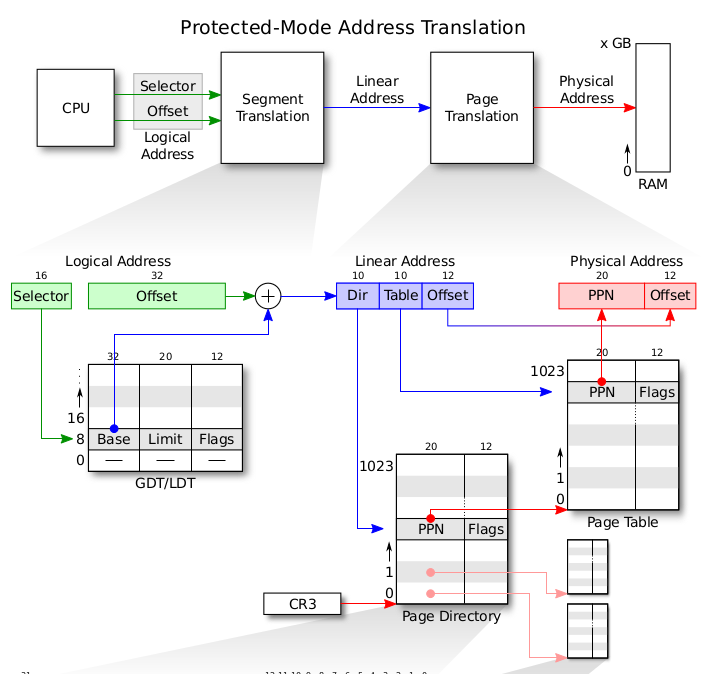
\includegraphics[scale=0.5]{LogicalAddrToPhysicAddr.png}
\par
这个图片介绍了如何从虚拟地址转化到物理地址的,这个图片对我做这个Lab非常有帮助。
\par
注意:在JOS中的segment translation在哪里?具体怎么实现的?如何使得OS能够正常运行?
\par
这个Exercise 4一定要时刻保持清醒的头脑,在于PAGE DIRECTORY,PAGE TABLE中表项均是保存的是物理地址,而操作系统内核无法跳过虚拟内存转化过程,因此操作系统进行内存地址操作的时候一定要使用虚拟内存。
\begin{subsubsection}{pddir\_walk()}
\par
pddir\_walk 将vitural memory对应的page table entry指针。如果不存在PAGE TABLE,则创建一个PAGE TABLE,并使得PAGE DIRECTORY对应项指向创建的PAGE TABLE。
\par
特别要注意pgdir中的所有项的中的PPN都是指的是物理地址,而内核无法避开使用虚拟内存转化的过程,因此在对指针进行取值操作的时候指针一定是要是指向虚拟地址的指针。这个地方我开始没考虑清楚,在该函数的return处的指针操作中没有加KADDR()而使用物理地址进行指针取值操作,导致疯狂Triple Fault。
\begin{lstlisting}[language=C]
pte_t *
pgdir_walk(pde_t *pgdir, const void *va, int create)
{
    // cprintf("pgdir_walk\n");
    if (pgdir[PDX(va)] == 0 || (pgdir[PDX(va)] & PTE_P) == 0) {
        // page table is not exist
        if (create == false) return NULL;

        struct PageInfo * new_page = page_alloc(1);
        if (new_page == NULL) return NULL;      // allocation fails
        ++new_page->pp_ref;
        pgdir[PDX(va)] = page2pa(new_page) | PTE_P | PTE_W | PTE_U;
    }
    return (pte_t *)KADDR(PTE_ADDR(pgdir[PDX(va)])) + PTX(va);
}
\end{lstlisting}
\end{subsubsection}

\begin{subsubsection}{boot\_map\_region}
\par
boot\_map\_region 将[va, va+size)虚拟地址映射到物理地址[pa, pa+size)上。对于虚拟地址映射的物理地址,只需要更改虚拟地址对应的page table entry的PPN值对应物理地址的高20位即可。因此可以使用pgdir\_walk来进行取(创建)对应page table entry。之后更改对应的PPN即可。
\begin{lstlisting}[language=C]
static void
boot_map_region(pde_t *pgdir, uintptr_t va, size_t size, physaddr_t pa, int perm)
{
    // cprintf("boot_map_region\n");
	// size is a multiple of PGSIZE
    uintptr_t va_now;
    pte_t * pte;
    for (va_now = va; va_now != va + size; va_now += PGSIZE, pa += PGSIZE) {
        pte = pgdir_walk(pgdir, (void *)va_now, true);
        // 20 PPN, 12 flag
        *pte = pa | PTE_P | perm;
    }
}
\end{lstlisting}
\par
注意:一开始我在va\_now != va + size写成了va\_now < va + size,在Part3中一直wa,之后才发现是这里写错了。我原本以为uintptr\_t因为是unsigned int类型,所以在比较的时候会默认按照unsigned类型进行比较,不会造成问题。但是在Part 3的映射中,其中会使得va + size == $2^{32}$,而在32位机下就是等于0,这样在使用va\_now < va + size进行判断的时候就会恒为false,造成错误。
\end{subsubsection}

\begin{subsubsection}{page\_lookup}
\par
返回虚拟地址va映射到的Page,实际上就是Page的物理地址就是对应page table entry的PPN。再利用pa2page转化到对应的PageInfo即可。
\begin{lstlisting}[language=C]
struct PageInfo *
page_lookup(pde_t *pgdir, void *va, pte_t **pte_store)
{
    // cprintf("page_lookup\n");
	// Fill this function in
    pte_t * pte = pgdir_walk(pgdir, va, 0);
    if (pte == NULL || (*pte & PTE_P) == 0) return NULL;   // no page mapped at va
    if (pte_store != 0) {
        *pte_store = pte;
    }
    return pa2page(PTE_ADDR(*pte));
}
\end{lstlisting}
\end{subsubsection}

\begin{subsubsection}{page\_remove}
\par
删除虚拟地址va到物理地址的映射。需要做两部:第一删除对应page table entry的信息,第二删除(减少引用次数)映射的页。tlb\_invalidate是刷新TLB用,以防止因为cache导致错误的寻址。
\begin{lstlisting}[language=C]
void
page_remove(pde_t *pgdir, void *va)
{
    // cprintf("page_remove\n");
	// Fill this function in
    pte_t * pte;
    struct PageInfo * pg = page_lookup(pgdir, va, &pte);
    if (pg == NULL) return;
    page_decref(pg);
    if (pte != NULL) *pte = 0;
    tlb_invalidate(pgdir, va); 
}
\end{lstlisting}
\end{subsubsection}

\begin{subsubsection}{page\_insert}
\par
将虚拟地址va映射到页pp上,如果原本有了别的映射,则需要删除原有映射。特别注意原有映射和pp相同的时候,因此方法很简单,先找到va对应的page table entry,并先将pp的pp\_ref增加,然后删去va原来对应的page table entry对应的映射,这里就是一个小技巧,由于page\_move只是会减少引用次数,只有引用次数为0才会真正删除页。而我们先增加引用次数这样即使映射到相同的页也不会造成错误。
\begin{lstlisting}[language=C]
int
page_insert(pde_t *pgdir, struct PageInfo *pp, void *va, int perm)
{
    // cprintf("page_insert\n");
	// Fill this function in
    pte_t * pte = pgdir_walk(pgdir, va, true);
    if (pte == NULL) return -E_NO_MEM;
    ++pp->pp_ref;
    if (*pte & PTE_P) {
        page_remove(pgdir, va);
    }
    *pte = page2pa(pp) | perm | PTE_P;        
	return 0;
}
\end{lstlisting}
\end{subsubsection}

\end{subsection}

\end{section}

\begin{section}{Part 3: Kernel Address Space}
\begin{subsection}{Exercise 5}
\par
在建立新的页寻址的时候,我们需要建立好新的映射。这样当我们将cr3指向新的Page Directory的时候就可以立即使用新的页寻址了。
\par
JOS将ULIM以上的部分都作为Kernel的部分,不允许用户访问,用户只能访问和使用ULIM一下的部分\par
按照JOS的要求:\par
1、[UPAGES, UPAGES + sizeof(PAGE))将会映射到[pages, pages + sizeof(PAGE))以用于页面管理。 \par
2、[KSTACKTOP-KSTKSIZE, KSTACKTOP) 将会映射到内核栈的实际物理地址,即在内核编译时.data预留的一段区域,[bootstack, bootstacktop)。但是并不是所有都用于实际的栈中,栈有一部分将会作为guard page,以防止内核栈溢出造成内核代码或数据的破坏,因此需要预留防止溢出的区域,并且这段区域不映射,当使用这个区域的时候将会造成page fault,因此来保护操作系统内核。\par
3、[KERNBASE, $2^{32}$) 将会映射到 [0, ...)。其中,这个映射直接保证了JOS之后启用新的页寻址,不会导致内核虚拟地址无法转化到实际的物理地址(内核的虚拟地址与实际地址仅相差KERNBASE)。\par

\begin{subsubsection}{map 'pages'}
\begin{lstlisting}[language=C]
    boot_map_region(kern_pgdir, 
                    UPAGES, 
                    ROUNDUP(npages * sizeof(struct PageInfo), PGSIZE), 
                    PADDR(pages),
                    PTE_U);
\end{lstlisting}
\end{subsubsection}

\begin{subsubsection}{map 'bootstack'}
\begin{lstlisting}[language=C]
	boot_map_region(kern_pgdir,
                    KSTACKTOP-KSTKSIZE,
                    KSTKSIZE,
                    PADDR(bootstack),
                    PTE_W);
\end{lstlisting}
\end{subsubsection}
\begin{subsubsection}{map all of physical memory}
\begin{lstlisting}[language=C]
	boot_map_region(kern_pgdir,
                    KERNBASE,
                    -KERNBASE,
                    0,
                    PTE_W); 
   // in 32-bit system, 2^32 - KERNBASE = - KERNBASE
\end{lstlisting}
\end{subsubsection}

\end{subsection}

\begin{subsection}{Question}
\begin{subsubsection}{Q2}
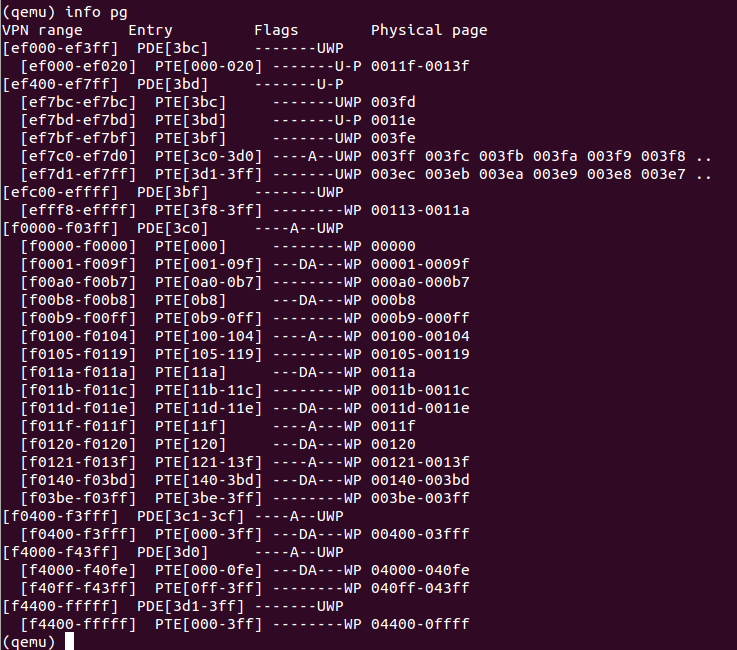
\includegraphics[scale=0.5]{Ex5infopg.png}
\par
利用qemu的info pg,我们可以知道虚拟内存到物理内存的映射情况。
\begin{center}
    \begin{tabular}{ | l | l | l |}
    \hline
           Base Virtual Address & Points to (logically): 	\\ \hline
           ef000000-ef020fff   &  pages 						\\ \hline
           ef7bc000-ef7fffff   &  recursively insert itself     \\ \hline
           efff8000-efffffff   &  Stack 							\\ \hline
           f0000000-ffffffff   &  KERN and Other \\   
    \hline
    \end{tabular}
\end{center}
\end{subsubsection}

\begin{subsubsection}{Q3}
\par
在PDE和PTE的flags位中,由R/W位,U/S位控制是否可写,是否需要supervisor权限。这样即使是使用同样的地址空间可以避免用户使用错误的地址进行读写。
\end{subsubsection}

\begin{subsubsection}{Q4}
\par
JOS对于管理PageInfo的大小至多为PTSIZE,在mmu.h中可知PTSIZE=4M,而每个PageInfo需要8-byte,因此至多有512k个页,因此最多支持512k * 4M = 2G的物理内存。
\end{subsubsection}

\begin{subsubsection}{Q5}
\par
需要1页的Page directory,Page directory共1024项,每项需要一个页,因此需要4M + 4K来管理内存。由Q4,PageInfo的管理最多使用PTSIZE,因此一共需要8M+4K来管理内存。
\end{subsubsection}

\begin{subsubsection}{Q6}
\par
从entrypgdir.c中可以看出,页将[0, 4MB)和[KERNBASE, KERNBASE + 4MB)均映射到了物理地址的[0, 4MB)因此在开启页之后即使为low eip,也能继续运行。知道jmp到高地才真正运行在eip > KERNBASE上。由于无法直接更改eip,因此我们需要跳转语句来实现eip的执行到高位地址上,而在开启页到跳转期间依然是low eip执行,为了保证寻址正确,因此需要将虚拟地址的[0, 4MB)映射到物理地址的[0, 4MB)上。
\end{subsubsection}


\end{subsection}

\begin{subsection}{Challenge 1:}
\par
PTE\_PS即使用大页直接映射4MB的空间,不需要二级页表,仅仅使用一级页表,这就减少了页表空间的开销,而且可以大大增加TLB的命中率。具体的映射方式在Intel手册上第三章有介绍,简单来说就是下面这张图:
\par:
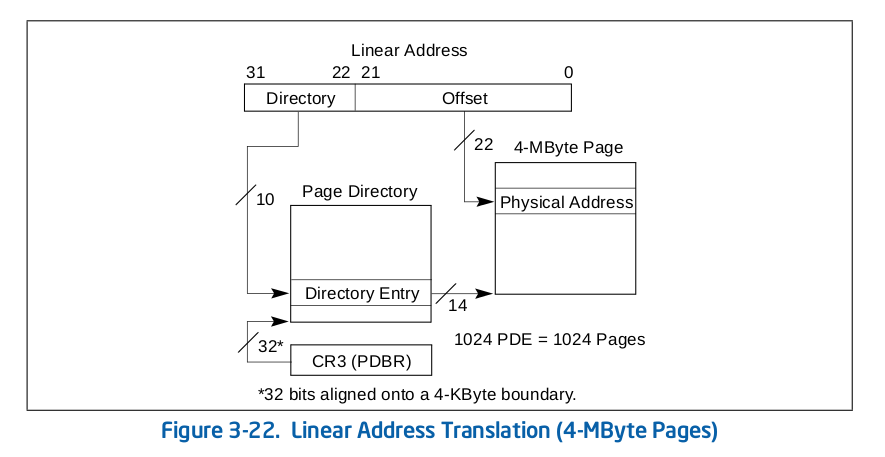
\includegraphics[scale=0.5]{4Mpage.png}
\par
如何更改使得可以使用4M页的映射呢?实际上就是Page Directory的PDE中设置PS位置为1,而且非常方便了不需要分配Page Table,直接设置PPN就可以了。这么方便的事情我觉得还是需要写写看的。依次观察什么地方需要更改:
\par
page\_init, page\_alloc, page\_free, page\_decref, page\_insert, page\_remove, page\_walk都没有关系。似乎boot\_map\_region还有点可能更改,也省得再写一个插入了,直接更改boot\_map\_region好了。
\par
具体更改方式也很简单,根据条件判断一下,具体实现根据上面的图即可。
\begin{lstlisting}[language=C]
static void
boot_map_region(pde_t *pgdir, uintptr_t va, size_t size, physaddr_t pa, int perm)
{
    // cprintf("boot_map_region\n");
	// size is a multiple of PGSIZE
    uintptr_t va_now;
    pte_t * pte;
    if (perm & PTE_PS) {
    	// 4M mapping
    	for (va_now = ROUNDDOWN(va, PGSIZE_PS); va_now != ROUNDUP(va + size, PGSIZE_PS); va_now += PGSIZE_PS, pa += PGSIZE_PS) {
    		pte = &pgdir[PDX(va_now)];
    		*pte = pa | PTE_P | PTE_PS | perm;
    	} 
    } else {
    	// 4K mapping
    	for (va_now = va; va_now != va + size; va_now += PGSIZE, pa += PGSIZE) {
        	pte = pgdir_walk(pgdir, (void *)va_now, true);
        	// 20 PPN, 12 flag
        	*pte = pa | PTE_P | perm;
    	}
	}
}
\end{lstlisting}
\par
测试的话,我只将kernel的高于KERNBASE的地址都用4M大页映射,但是这样通不过check的KERNBASE + i == i的测试,于是我把check也改了。。。好邪恶的感觉。
\begin{lstlisting}[language=C]
// in mem_init
    boot_map_region(kern_pgdir,
                    KERNBASE,
                    -KERNBASE,
                    0,
                    PTE_W | PTE_PS); 
                    
                    
static physaddr_t
check_va2pa(pde_t *pgdir, uintptr_t va)
{
	pte_t *p;

	pgdir = &pgdir[PDX(va)];
	if (!(*pgdir & PTE_P))
		return ~0;
	if (*pgdir & PTE_PS) {
		// 4M page
		// uintptr_t tmp = ((*pgdir) & (0xffc00000)) | (va & (~0xffc00000));
		// cprintf("%u\n", tmp);
		return PTE_ADDR(((*pgdir) & (0xffc00000)) | (va & (~0xffc00000)));
	}
	p = (pte_t*) KADDR(PTE_ADDR(*pgdir));
	if (!(p[PTX(va)] & PTE_P))
		return ~0;
	return PTE_ADDR(p[PTX(va)]);
}
\end{lstlisting}
\par
但是,竟然运行Triple fault,调了很久似乎没有发现错误,后来在马林同学的提醒才发现我忘记设置开关了。
\par
在cr4中的bit 4是Page Size Extension位,表示可以启用4M的大页寻址。因此在导入新的页目录前将cr4开启Page Size Extension就可以了。即:
\begin{lstlisting}[language=C]
	lcr4(CR4_PSE);					// Open Size Page Extension
	lcr3(PADDR(kern_pgdir));
\end{lstlisting}
\par
实验效果如下:
\paragraph{•}
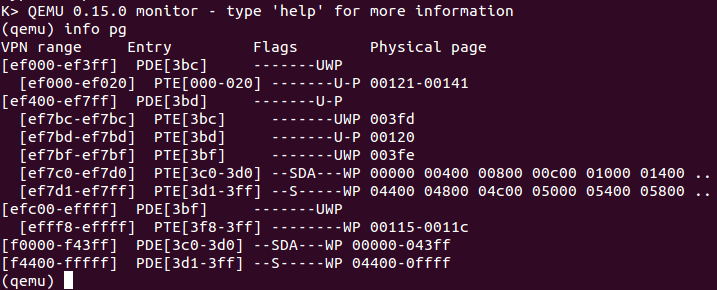
\includegraphics[scale=0.5]{PSE.png}
\par
其中Flag中标注为S即使用了4M大页查询。
\end{subsection}

\begin{subsection}{Challenge 2:}
\begin{subsubsection}{ ShowMappings }
\par
showmappings为显示虚拟地址对应的物理地址。showmappings只需要利用pgdir\_walk到对应的page table entry即可。
\begin{lstlisting}[language=C]
int
mon_showmappings(int argc, char **argv, struct Trapframe *tf)
{
    if (argc != 3) {
        cprintf("Command should be: showmappings [addr1] [addr2]\n");
        cprintf("Example: showmappings 0x3000 0x5000\n");
    } else {
        uint32_t laddr = strtol(argv[1], NULL, 0);
        uint32_t haddr = strtol(argv[2], NULL, 0);
        if (laddr > haddr) {
            haddr ^= laddr;
            laddr ^= haddr;
            haddr ^= laddr;
        }
        laddr = ROUNDDOWN(laddr, PGSIZE);
        haddr = ROUNDUP(haddr, PGSIZE);
        cprintf("0x%08x - 0x%08x\n", laddr, haddr);
        
        uint32_t now;
        pte_t *pte;
        for (now = laddr; now != haddr; now += PGSIZE) {
            cprintf("[ 0x%08x, 0x%08x ) -> ", now, now + PGSIZE); 
            pte = pgdir_walk(kern_pgdir, (void *)now, 0);
            if (pte == 0 || (*pte & PTE_P) == 0) {
                cprintf(" no mapped \n");
            } else {
                cprintf("0x%08x ", PTE_ADDR(*pte));
                if (*pte & PTE_U) cprintf(" user       ");
                else cprintf(" supervisor ");
                if (*pte & PTE_W) cprintf(" RW ");
                else cprintf(" R ");
                cprintf("\n");
            }
        }
    }
    return 0;
}
\end{lstlisting}
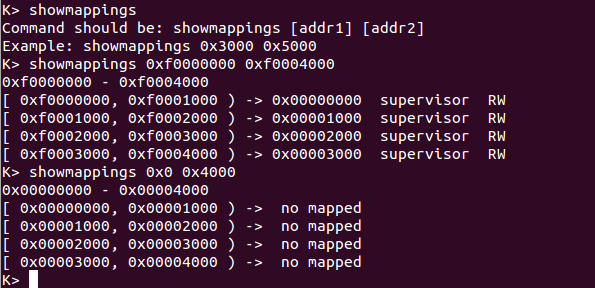
\includegraphics[scale=0.5]{showmappings.png}
\end{subsubsection}

\begin{subsubsection}{ SetPermission }
\par
对于set permission类似直接通过pgdir\_walk更改即可。
\begin{lstlisting}[language=C]
int
mon_setpermission(int argc, char **argv, struct Trapframe *tf)
{
    if (argc != 5) { 
        cprintf("Command should be: setpermissions [virtual addr] [W (0/1)] [U (0/1)] [P (0/1)]\n");
        cprintf("Example: setpermissions 0x0 1 0 1\n");
    } else {
        uint32_t addr = strtol(argv[1], NULL, 0);
        uint32_t perm = 0;
        if (argv[2][0] == '1') perm |= PTE_W;
        if (argv[3][0] == '1') perm |= PTE_U;
        if (argv[4][0] == '1') perm |= PTE_P;
        addr = ROUNDUP(addr, PGSIZE);
        pte_t *pte = pgdir_walk(kern_pgdir, (void *)addr, 0);
        if (pte != NULL) {
            cprintf("0x%08x -> pa: 0x%08x\n old_perm: ", addr, PTE_ADDR(*pte));
            if (*pte & PTE_W) cprintf("RW"); else cprintf("R-");
            if (*pte & PTE_U) cprintf("U"); else cprintf("S");
            if (*pte & PTE_P) cprintf("P"); else cprintf("-");
            cprintf("  --> new_perm: ");
            *pte = PTE_ADDR(*pte) | perm;     
            if (*pte & PTE_W) cprintf("RW"); else cprintf("R-");
            if (*pte & PTE_U) cprintf("U"); else cprintf("S");
            if (*pte & PTE_P) cprintf("P"); else cprintf("-");
            cprintf("\n");
        } else {
            cprintf(" no mapped \n");
        }
    }
    return 0;
}
\end{lstlisting}
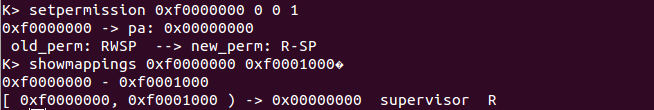
\includegraphics[scale=0.5]{setpermission.png}
\end{subsubsection}

\begin{subsubsection}{ Dump }
\par
对于dump,如果是查询虚拟内存的内容,则非常简单,直接输出即可。但是问题在于如何得到物理地址的内容,这对于已经建立好了页映射的操作系统来说是困难的,而对于JOS,由于已经清楚地知道其物理内存和虚拟内存的映射关系,因此我根据映射关系来写就可以解决了。
\par
pa\_con(addr, *value)为查找物理地址为addr的4-byte的值,返回是否存在值,如果存在则值保存在value。
\begin{lstlisting}[language=C]
bool
pa_con(uint32_t addr, uint32_t * value)
{
    // get value in addr(physical address)
    // if no page mapped in addr, return false;
    if (addr >= PADDR(pages) && addr < PADDR(pages) + PTSIZE) {
        // PageInfo
        *value = *(uint32_t *)(UPAGES + (addr - PADDR(pages)));
        return true;
    }
    if (addr >= PADDR(bootstack) && addr < PADDR(bootstack) + KSTKSIZE) {
        // kernel stack
        *value = *(uint32_t *)(KSTACKTOP - KSTKSIZE + (addr - PADDR(bootstack)));
        return true;
    }
    if (addr < -KERNBASE) {
        // Other
        *value = *(uint32_t *)(addr + KERNBASE);
        return true;
    }
    // Not in virtual memory mapped.
    return false;
}

int
mon_dump(int argc, char **argv, struct Trapframe *tf)
{
    if (argc != 4) {
        cprintf("Command should be: dump [v/p] [addr1] [addr2]\n");
        cprintf("Example: dump v 0xf0000000 0xf0000010\n");
        cprintf("         dump contents in virtual address [0xf0000000, 0xf0000010)\n");
    } else {
        uint32_t laddr = strtol(argv[2], NULL, 0);
        uint32_t haddr = strtol(argv[3], NULL, 0);
        if (laddr > haddr) {
            haddr ^= laddr;
            laddr ^= haddr;
            haddr ^= laddr;
        }
        laddr = ROUNDDOWN(laddr, 4);
        haddr = ROUNDDOWN(haddr, 4);
        if (argv[1][0] == 'v') {
            // virtual address
            uint32_t now;
            pte_t * pte;
            for (now = laddr; now != haddr; now += 4) {
                if (now == laddr || ((now & 0xf) == 0)) {
                    if (now != laddr) cprintf("\n"); 
                    cprintf("0x%08x:  ", now);
                }
                pte = pgdir_walk(kern_pgdir, (void *)ROUNDDOWN(now, PGSIZE), 0);
                if (pte && (*pte & PTE_P)) 
                    cprintf("0x%08x  ", *((uint32_t *)now));
                else
                    cprintf("--------  ");
            }
            cprintf("\n");
        } else {
            // physical address
            uint32_t now, value;
            for (now = laddr; now != haddr; now += 4) {
                if (now == laddr || ((now & 0xf) == 0)) {
                    if (now != laddr) cprintf("\n");
                    cprintf("0x%08x:  ", now);
                }
                if (pa_con(now, &value)) {
                    cprintf("0x%08x  ", value);
                } else
                    cprintf("----------  ");
            }
            cprintf("\n");
        }
    }
    return 0;
}
\end{lstlisting}
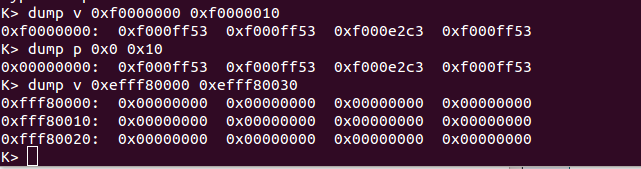
\includegraphics[scale=0.5]{dump.png}
\end{subsubsection}

\begin{subsubsection}{ my tool for debug }
\par
我写了一个查看page directory项的函数
\begin{lstlisting}[language=C]
int 
mon_kernelpd(int argc, char **argv, struct Trapframe *tf)
{
    if (argc != 2) {
        cprintf("Command should be: kernelpd [entry_num]\n");
        cprintf("Example: kernelpd 0x01\n");
        cprintf("         show kernel page directory[1] infomation \n");
    } else {
        uint32_t id = strtol(argv[1], NULL, 0);
        if (0 > id || id >= 1024) {
            cprintf("out of entry num, it should be in [0, 1024)\n");
        } else {
            cprintf("pgdir[%d] = 0x%08x\n", id, (uint32_t)kern_pgdir[id]);
        }
    }
    return 0;
}
\end{lstlisting}
\par
没什么好说的
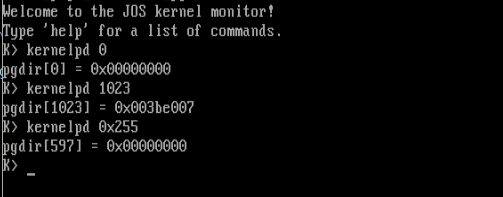
\includegraphics[scale=0.5]{kernelpd.png}
\end{subsubsection}

\end{subsection}

\begin{subsection}{Challenge 3:}
暂时没查到相关资料,对于kernel在内核态和用户态的转化也不太清楚,等过段时间再回来做好了。。。
\end{subsection}

\begin{subsection}{Challenge 4:}
\par
可以使用Buddy Systems,基本思想是有大小为$2^m$的空间,每次请求某个大小都会分割离请求值向上取最近的2的次幂的大小。对于请求分配$2^k$大小的空间,首先会找到最小的空闲块,大小为$2^j$,满足$j>=k$,如果$j=k$那么很好,则可以直接分配,否则我们递归对半分割$2^j$的空间,直到出现$2^k$大小的空间。对于清楚分配的空间也很简单,如果已经有相同大小的空闲块,则合并为一个更大的空闲块,直到不存在相同大小的空闲块。这些操作都可以利用二进制数进行位运算来进行,使得分配合并速度变快,缺点在于会有很多内部碎片。
\end{subsection}

\end{section}

\begin{section}{ Something Interesting... }
\begin{subsection}{ Mem }
\par
 Lab1可知初始的页将[0, 4M) , [KERNBASE, KERNBASE + 4M) 映射到了[0, 4M)的地方。而我们有16639个可以分配页,最大的可用的地址显然超过了4M也就是没被映射,而在boot\_map\_region里面却使用了该地址的解引用( *pte = ....),为什么没有出错?
\par
因为在check\_page\_free\_list()里面他帮我们做了剔除没有被原来4M的页的操作。 太邪恶了,我还思索了很久。
\end{subsection}

\begin{subsection}{ Self-Reference in Page Directory }
\par
在mem\_init(void)中有这样一句话:
\begin{lstlisting}[language=C]
	//////////////////////////////////////////////////////////////////////
	// Recursively insert PD in itself as a page table, to form
	// a virtual page table at virtual address UVPT.
	// (For now, you don't have understand the greater purpose of the
	// following line.)

	// Permissions: kernel R, user R
	kern_pgdir[PDX(UVPT)] = PADDR(kern_pgdir) | PTE_U | PTE_P;
\end{lstlisting}
\par
就是在UVPT的page table映射指向了自己,我实在不清楚这样做的意义在哪里?唯一可以想到的只有这个地方可以让用户态的进程只读这块。好吧,我现在还不知道答案。。。
\end{subsection}

\end{section}

\begin{section}{ Summary }
\par
这个Lab我估计一共花了将近30个小时,很多地方都是自己突然想不清对应关系导致的,特别是什么区别合适使用物理内存,虚拟内存的时候。通过这个Lab我也深刻理解了操作系统中的页寻址到底是什么回事,其背后的实现。
\par
最后感谢马林同学在我challenge 1中一直不知道哪里错的时候提醒我是不是没设cr4的开关。还有感谢毛景树同学提供给我的Latex的模板!
\end{section}


\end{document}



















